\documentclass[11pt]{article}
\usepackage[margin=1in]{geometry}
\usepackage{amsmath,amssymb}
\usepackage{siunitx}
\usepackage{physics}
\usepackage{tikz}
\usetikzlibrary{arrows.meta,angles,quotes,calc,decorations.pathmorphing,decorations.markings,patterns}
\usepackage{enumitem}
\sisetup{per-mode=symbol}

\newcommand{\ans}[1]{\boxed{\displaystyle #1}}

\title{PHYS 121 --- HW6 Solutions}
\author{Juntang Wang}

\begin{document}
\maketitle
\setlist[itemize]{noitemsep,topsep=2pt}

%%%%%%%%%%%%%%%%%%%%%%%%%%%%%%%%%%%%%%%%%%%%%%%%%%%%%%%%
\section*{Q1. Temperature of a pendulum (4+4 pts)}

Period of a simple pendulum (small oscillations):
\[
T = 2\pi\sqrt{\frac{L}{g}} \quad\Rightarrow\quad
\frac{dT}{T} = \frac{1}{2}\frac{dL}{L}.
\]
Thermal expansion: \(dL = \alpha L\,dT\), so
\[
\frac{dT_{\text{period}}}{T}
 = \frac{1}{2}\frac{dL}{L}
 = \frac{1}{2}\alpha\,dT.
\]

If the clock is correct at \(T_{\rm cal}\) and the room is at
\(T_{\rm room}=T_{\rm cal}+\Delta T\) with \(\Delta T>0\),
then \(L\) increases, so \(T\) increases and the clock \emph{runs slow}
(falls behind).

Over one true day \(t_{\text{day}}=86400\,\text{s}\), the fractional
error in the time kept by the clock is the same:
\[
\frac{\Delta t}{t_{\text{day}}}
 = \frac{1}{2}\alpha\Delta T
 \quad\Rightarrow\quad
\Delta t = \frac{1}{2}\alpha\Delta T\;t_{\text{day}}.
\]
Since \(T\) is larger, this is a \emph{loss} of time:
\[
\ans{\Delta t_{\text{(slow)}} =
 \frac{1}{2}\alpha\Delta T\,(86400\ \text{s/day})}.
\]

\bigskip
\noindent\textbf{Required sketch:}
\begin{center}
  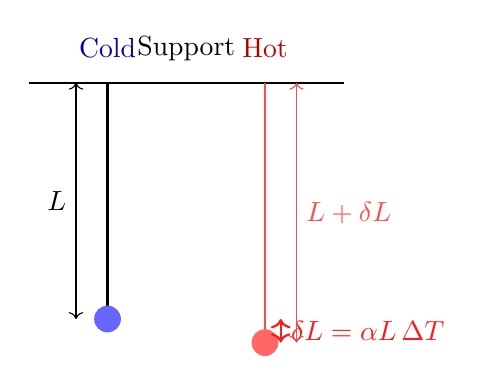
\begin{tikzpicture}[scale=1.0]
    % Beam / support
    \draw[thick] (-2,0) -- (2,0);
    \node[above] at (0,0.15) {Support};
  
    % Cold pendulum (left)
    \draw[thick] (-1,0) -- (-1,-3);
    \fill[blue!60] (-1,-3) circle (0.17);
    \draw[<->] (-1.4,0) -- (-1.4,-3) node[midway,left] {$L$};
    \node[above,blue!70!black] at (-1,0.2) {Cold};
  
    % Hot pendulum (right)
    \draw[thick,red!70] (1,0) -- (1,-3.3);
    \fill[red!60] (1,-3.3) circle (0.17);
    \draw[<->,red!70] (1.4,0) -- (1.4,-3.3) node[midway,right] {$L+\delta L$};
  
    % Delta L indicator
    \draw[<->,red!90,thick] (1.2,-3) -- (1.2,-3.3)
      node[midway,right] {$\delta L = \alpha L\,\Delta T$};
  
    \node[above,red!70!black] at (1,0.2) {Hot};
  \end{tikzpicture}
  \end{center}

%%%%%%%%%%%%%%%%%%%%%%%%%%%%%%%%%%%%%%%%%%%%%%%%%%%%%%%%
\section*{Q2. Estimate Earth's temperature (2+3+3+1 pts)}

Solar constant at Earth's orbit: \(S\simeq\SI{1370}{W/m^2}\).
Stefan--Boltzmann constant: \(\sigma\).

\subsection*{(a) Intercepted power}
The Earth intercepts sunlight over its geometric cross section:
\[
P_{\text{in}} = S\;\pi R^2.
\]

If it is a blackbody at temperature \(T\), it radiates from its whole
surface area \(4\pi R^2\):
\[
P_{\text{out}} = 4\pi R^2\sigma T^4.
\]

Equating \(P_{\text{in}} = P_{\text{out}}\) gives
\[
S\pi R^2 = 4\pi R^2\sigma T^4
\quad\Rightarrow\quad
T = \left(\frac{S}{4\sigma}\right)^{1/4}
 \approx \ans{\SI{279}{K}}.
\]

\subsection*{(b) Including albedo}
With albedo \(A=0.3\), only a fraction \((1-A)\) is absorbed:
\[
P_{\text{in}} = (1-A)S\pi R^2.
\]
Set equal to \(4\pi R^2\sigma T^4\):
\[
(1-A)S\pi R^2 = 4\pi R^2\sigma T^4
\quad\Rightarrow\quad
T = \left(\frac{(1-A)S}{4\sigma}\right)^{1/4}
 \approx \ans{\SI{255}{K}}.
\]

\subsection*{(c) Role of greenhouse effect}
Observed mean surface temperature is about \(\SI{288}{K}\), well above
\(\SI{255}{K}\). Thus atmospheric greenhouse warming is
important: 
\[
\ans{\text{yes, the greenhouse effect is significant}}.
\]

\subsection*{(d) Dependence on Earth's area}
Both absorbed and emitted powers scale as \(R^2\), so they cancel in the
balance. Therefore
\[
\ans{T\ \text{is independent of Earth's radius (area) in this model}.}
\]

%%%%%%%%%%%%%%%%%%%%%%%%%%%%%%%%%%%%%%%%%%%%%%%%%%%%%%%%
\section*{Q3. Unreasonable results? H\textsubscript{2}S speeds (3+5 pts)}

Molar mass of \(\mathrm{H_2S}\): \(M = \SI{31.4}{g/mol} = 0.0314\,\si{kg/mol}\).

\subsection*{(a) Average speed}
For an ideal gas, the mean speed is
\[
\bar v = \sqrt{\frac{8RT}{\pi M}}.
\]
At \(T=\SI{250}{K}\),
\[
\bar v
 = \sqrt{\frac{8(8.314)(250)}{\pi(0.0314)}}
 \approx \ans{\SI{4.1e2}{m/s}}.
\]

\subsection*{(b) Reliability of this result}
At \(\SI{250}{K}\) and realistic pressures, \(\mathrm{H_2S}\) is far from an
ideal, nearly noninteracting gas: it has strong intermolecular
attractions and a relatively high boiling point. The assumptions of the
Maxwell--Boltzmann distribution (point particles, negligible
interactions except elastic collisions, ideal equation of state) are
poor. Thus the numerical speed is much less reliable than for ideal,
monoatomic gases; real interactions and non-ideality matter.

%%%%%%%%%%%%%%%%%%%%%%%%%%%%%%%%%%%%%%%%%%%%%%%%%%%%%%%%
\section*{Q4. Airtight water dispenser (10 pts)}

Given: Cross-section \(A = 25\,\text{cm} \times 10\,\text{cm} = \SI{0.025}{m^2}\),
total height \(H = \SI{20}{cm} = \SI{0.20}{m}\),
initial water level \(h_0 = 20 - 3.5 = \SI{16.5}{cm} = \SI{0.165}{m}\),
initial air pressure \(P_{0,\text{air}} = \SI{1.00}{atm} = \SI{1.013e5}{Pa}\),
water density \(\rho = \SI{1000}{kg/m^3}\),
temperature constant (isothermal).

\subsection*{(a) Pressure at bottom}
\[
P_{\text{bottom}} = P_{\text{air}} + \rho g h.
\]
For gauge pressure = 0, \(P_{\text{bottom}} = P_{\text{atm}} = \SI{1.00}{atm}\).

\subsection*{(b) Isothermal air relation}
For isothermal air: \(P_{\text{air}} V_{\text{air}} = \text{constant}\).

Initial: \(V_{0,\text{air}} = A(H - h_0) = A(0.20 - 0.165) = \SI{8.75e-4}{m^3}\).

Final: \(V_{\text{air}} = A(H - h)\), so
\[
P_{\text{air}} = P_{0,\text{air}} \frac{V_{0,\text{air}}}{V_{\text{air}}}
= P_{0,\text{air}} \frac{H - h_0}{H - h}.
\]

\subsection*{(c) Final water height and volume}
At equilibrium: \(P_{\text{bottom}} = P_{\text{air}} + \rho g h = P_{\text{atm}}\).

Substituting:
\[
P_{0,\text{air}} \frac{H - h_0}{H - h} + \rho g h = P_{\text{atm}}.
\]

With \(P_{0,\text{air}} = P_{\text{atm}}\), this simplifies to:
\[
P_{\text{atm}} \frac{H - h_0}{H - h} + \rho g h = P_{\text{atm}}.
\]

Rearranging:
\[
P_{\text{atm}} \left(\frac{H - h_0}{H - h} - 1\right) = -\rho g h,
\]
\[
P_{\text{atm}} \frac{h - h_0}{H - h} = -\rho g h.
\]

Multiplying both sides by \((H - h)\):
\[
P_{\text{atm}}(h - h_0) = -\rho g h (H - h).
\]

Rearranging: \(h_0 = h + \frac{(H-h)\rho g h}{P_{\text{atm}}}\).

This gives a quadratic in \(h\):
\[
\frac{\rho g}{P_{\text{atm}}} h^2 - \left(1 + \frac{H\rho g}{P_{\text{atm}}}\right)h + h_0 = 0.
\]

Using \(P_{\text{atm}} = \SI{1.013e5}{Pa}\), \(\rho g = \SI{9800}{N/m^3}\), \(H = \SI{0.20}{m}\), \(h_0 = \SI{0.165}{m}\):
\[
0.0967 h^2 - 1.0193 h + 0.165 = 0.
\]

Solving: \(h = \SI{0.1644}{m} = \SI{16.4}{cm}\).

Volume of water flowed out:
\[
\Delta V = A(h_0 - h) = 0.025 \times (0.165 - 0.1644) = \ans{\SI{1.5e-5}{m^3} = \SI{15}{cm^3}}.
\]

\noindent\textbf{Required drawing:}
\begin{center}
  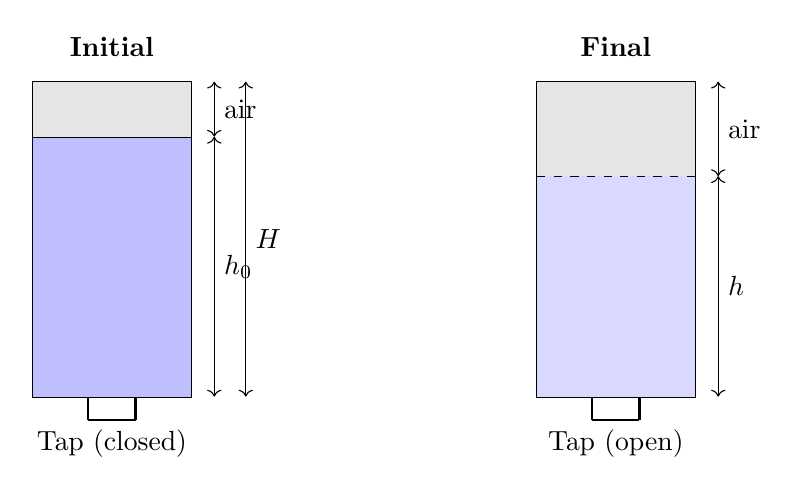
\begin{tikzpicture}[scale=1.0]
    % Common dimensions for both sketches
    \def\W{2}   % width
    \def\H{4}   % total height
  
    % ---- Initial state (left) ----
    \begin{scope}[xshift=-3.2cm]
      % Outer walls
      \draw[thick] (0,0) rectangle (\W,\H);
      % Water level
      \def\hwater{3.3}
      \fill[blue!25] (0,0) rectangle (\W,\hwater);
      \draw[thick] (0,\hwater) -- (\W,\hwater);
      % Air pocket
      \fill[gray!20] (0,\hwater) rectangle (\W,\H);
  
      % Labels
      \draw[<->] (\W+0.3,0) -- (\W+0.3,\hwater)
        node[midway,right] {$h_0$};
      \draw[<->] (\W+0.3,\hwater) -- (\W+0.3,\H)
        node[midway,right] {air};
      \draw[<->] (\W+0.7,0) -- (\W+0.7,\H)
        node[midway,right] {$H$};
  
      % Tap
      \draw[thick] (0.7,-0.3) -- (1.3,-0.3);
      \draw[thick] (0.7,-0.3) -- (0.7,0);
      \draw[thick] (1.3,-0.3) -- (1.3,0);
      \node[below] at (1.0,-0.3) {Tap (closed)};
  
      \node[above] at (1,\H+0.2) {\textbf{Initial}};
    \end{scope}
  
    % ---- Final state (right) ----
    \begin{scope}[xshift=3.2cm]
      % Outer walls
      \draw[thick] (0,0) rectangle (\W,\H);
      % Final water level (slightly lower)
      \def\hfinal{2.8}
      \fill[blue!15] (0,0) rectangle (\W,\hfinal);
      \draw[thick,dashed] (0,\hfinal) -- (\W,\hfinal);
      % Air pocket
      \fill[gray!20] (0,\hfinal) rectangle (\W,\H);
  
      % Labels
      \draw[<->] (\W+0.3,0) -- (\W+0.3,\hfinal)
        node[midway,right] {$h$};
      \draw[<->] (\W+0.3,\hfinal) -- (\W+0.3,\H)
        node[midway,right] {air};
  
      % Tap
      \draw[thick] (0.7,-0.3) -- (1.3,-0.3);
      \draw[thick] (0.7,-0.3) -- (0.7,0);
      \draw[thick] (1.3,-0.3) -- (1.3,0);
      \node[below] at (1.0,-0.3) {Tap (open)};
  
      \node[above] at (1,\H+0.2) {\textbf{Final}};
    \end{scope}
  \end{tikzpicture}
  \end{center}

%%%%%%%%%%%%%%%%%%%%%%%%%%%%%%%%%%%%%%%%%%%%%%%%%%%%%%%%
\section*{Q5. Adiabatic process (3+3+3+3 pts)}

Given: \(n = 1\,\text{mol}\), \(V_1 = \SI{1.0e-2}{m^3}\),
\(P_1 = \SI{2.0e5}{N/m^2}\), \(V_2 = \SI{5.0e-3}{m^3}\),
monatomic gas (\(\gamma = 5/3\)), adiabatic compression.

\subsection*{(a) Initial temperature}
From ideal gas law: \(P_1 V_1 = nRT_1\),
\[
T_1 = \frac{P_1 V_1}{nR} = \frac{2.0 \times 10^5 \times 1.0 \times 10^{-2}}{1 \times 8.314}
= \ans{\SI{241}{K}}.
\]

\subsection*{(b) Final temperature}
For adiabatic process: \(T V^{\gamma-1} = \text{constant}\), so
\[
T_2 = T_1 \left(\frac{V_1}{V_2}\right)^{\gamma-1}
= 241 \left(\frac{1.0 \times 10^{-2}}{5.0 \times 10^{-3}}\right)^{2/3}
= 241 \times 2^{2/3} \approx \ans{\SI{382}{K}}.
\]

\subsection*{(c) Work done on gas}
For adiabatic process: \(W = \frac{nR}{\gamma-1}(T_1 - T_2)\),
\[
W = \frac{1 \times 8.314}{5/3 - 1}(241 - 382)
= \frac{8.314}{2/3} \times (-141)
= \SI{1.76e3}{J}.
\]
Work done \emph{on} the gas is \ans{+\SI{1.76e3}{J}}.

\subsection*{(d) Change in internal energy}
For monatomic ideal gas: \(\Delta U = \frac{3}{2}nR(T_2 - T_1)\),
\[
\Delta U = \frac{3}{2} \times 1 \times 8.314 \times (382 - 241)
= \ans{\SI{1.76e3}{J}}.
\]

\noindent\textbf{Required drawing:}
\begin{center}
  \begin{tikzpicture}[scale=1.0]
    % Axes
    \draw[->] (0,0) -- (6,0) node[right] {$V$};
    \draw[->] (0,0) -- (0,4) node[above] {$P$};
  
    % Adiabatic curve (schematic)
    \draw[thick,blue]
      (4,1.0) to[out=160,in=-20] (2,3.0);
  
    % States
    \fill (4,1.0) circle (2pt) node[below right] {$1$};
    \fill (2,3.0) circle (2pt) node[above left] {$2$};
  
    % Guide lines
    \draw[gray,dashed] (4,0) -- (4,1.0) node[below] {$V_1$};
    \draw[gray,dashed] (2,0) -- (2,3.0) node[below] {$V_2$};
  
    % Arrow showing direction
    \draw[->,red,thick] (3.4,1.4) -- (2.6,2.4);
    \node[red,above] at (3.0,2.0) {adiabatic compression};
  \end{tikzpicture}
  \end{center}

%%%%%%%%%%%%%%%%%%%%%%%%%%%%%%%%%%%%%%%%%%%%%%%%%%%%%%%%
\section*{Q6. Inelastic collision heating (5+5 pts)}

Given: \(m_b = \SI{10}{g} = \SI{0.010}{kg}\),
\(v_{b,0} = \SI{200}{m/s}\),
\(m_p = \SI{2.0}{kg}\),
\(C_V = 3R\),
\(M = \SI{200}{g/mol} = \SI{0.200}{kg/mol}\).

\subsection*{(a) Mechanical energy dissipated}
Momentum conservation: \(m_b v_{b,0} = (m_b + m_p)v_f\),
\[
v_f = \frac{m_b v_{b,0}}{m_b + m_p} = \frac{0.010 \times 200}{2.01} = \SI{0.995}{m/s}.
\]

Initial kinetic energy: \(K_i = \frac{1}{2}m_b v_{b,0}^2 = \frac{1}{2} \times 0.010 \times 200^2 = \SI{200}{J}\).

Final kinetic energy: \(K_f = \frac{1}{2}(m_b + m_p)v_f^2 = \frac{1}{2} \times 2.01 \times 0.995^2 = \SI{0.996}{J}\).

Energy dissipated:
\[
\Delta E = K_i - K_f = 200 - 0.996 = \ans{\SI{199}{J}}.
\]

\subsection*{(b) Temperature increase}
Total mass: \(m_{\text{tot}} = m_b + m_p = \SI{2.01}{kg}\).

Number of moles: \(n = \frac{m_{\text{tot}}}{M} = \frac{2.01}{0.200} = \SI{10.05}{mol}\).

Heat capacity at constant volume: \(C_V = 3R = \SI{24.94}{J/(mol\cdot K)}\).

Total heat capacity: \(C_{V,\text{tot}} = n C_V = 10.05 \times 24.94 = \SI{250.6}{J/K}\).

Temperature increase:
\[
\Delta T = \frac{\Delta E}{C_{V,\text{tot}}} = \frac{199}{250.6} = \ans{\SI{0.794}{K}}.
\]

%%%%%%%%%%%%%%%%%%%%%%%%%%%%%%%%%%%%%%%%%%%%%%%%%%%%%%%%
\section*{Q7. A Star is Born (3+3+3+2 pts)}

Given: Initial radius \(R_i\), initial density \(\rho_i\),
opacity density \(\rho_1\), initial temperature \(T_1\),
adiabatic index \(\gamma = 7/5\).

\subsection*{(a) Radius at opacity}
Mass conservation: \(M = \frac{4}{3}\pi R_i^3 \rho_i = \frac{4}{3}\pi r_1^3 \rho_1\),
\[
r_1^3 = R_i^3 \frac{\rho_i}{\rho_1}
\quad\Rightarrow\quad
r_1 = R_i \left(\frac{\rho_i}{\rho_1}\right)^{1/3}.
\]

\subsection*{(b) Temperature scaling and \(r_2\)}
For adiabatic process: \(T V^{\gamma-1} = \text{constant}\), so
\[
T r^{3(\gamma-1)} = \text{constant}
\quad\Rightarrow\quad
T \propto r^{-3(\gamma-1)} = r^{-6/5}.
\]

At temperature \(T_2\):
\[
T_2 r_2^{6/5} = T_1 r_1^{6/5}
\quad\Rightarrow\quad
r_2 = r_1 \left(\frac{T_1}{T_2}\right)^{5/6}.
\]

\subsection*{(c) Numerical \(r_1\)}
With \(R_i = \SI{3.0e15}{m}\),
\(\rho_i = \SI{2.0e-14}{g/m^3} = \SI{2.0e-17}{kg/m^3}\),
\(\rho_1 = \SI{1.0e-7}{g/m^3} = \SI{1.0e-10}{kg/m^3}\):
\[
r_1 = 3.0 \times 10^{15} \left(\frac{2.0 \times 10^{-17}}{1.0 \times 10^{-10}}\right)^{1/3}
= 3.0 \times 10^{15} \times (2.0 \times 10^{-7})^{1/3}.
\]
\[
r_1 = 3.0 \times 10^{15} \times 5.848 \times 10^{-3}
= \ans{\SI{1.75e13}{m}}.
\]

\subsection*{(d) Numerical \(r_2\)}
With \(T_2 = \SI{2000}{K}\), and assuming \(T_1\) is the initial temperature
(typically around \(\SI{10}{K}\) for molecular clouds):
\[
r_2 = r_1 \left(\frac{T_1}{T_2}\right)^{5/6}
= 1.76 \times 10^{13} \left(\frac{T_1}{2000}\right)^{5/6}.
\]

If \(T_1 = \SI{10}{K}\):
\[
r_2 = 1.75 \times 10^{13} \times \left(\frac{10}{2000}\right)^{5/6}
= 1.75 \times 10^{13} \times (0.005)^{5/6}
\approx 1.75 \times 10^{13} \times 0.0121
\approx \ans{\SI{2.1e11}{m}}.
\]

%%%%%%%%%%%%%%%%%%%%%%%%%%%%%%%%%%%%%%%%%%%%%%%%%%%%%%%%
\section*{Q8. A process: piston + mass, adiabatic vs isothermal (3+4+4+3 pts)}

Given: \(n = 1\,\text{mol}\) He (monatomic, \(\gamma = 5/3\)),
\(T_1 = \SI{27}{\degreeCelsius} = \SI{300}{K}\),
\(P_1 = \SI{100.0}{kPa} = \SI{1.00e5}{Pa}\),
piston area \(A = \SI{0.0010}{m^2}\),
mass on piston \(m = \SI{2.0}{kg}\),
bath temperature \(T_{\text{bath}} = \SI{27}{\degreeCelsius} = \SI{300}{K}\),
and atmospheric pressure \(P_{\text{atm}} = P_1\).

Initial volume:
\[
V_1 = \frac{nRT_1}{P_1}
= \frac{1 \times 8.314 \times 300}{1.00 \times 10^5}
= \SI{0.0249}{m^3}.
\]

\subsection*{(a) Minimum volume during first dip}

When the mass is suddenly placed on the piston, the gas is compressed adiabatically (rapid process, no heat exchange).

The work done on the gas comes from:
\begin{itemize}
\item The added mass: pressure \(mg/A\) over area \(A\),
\item The atmosphere: pressure \(P_{\text{atm}}\).
\end{itemize}

Total external pressure on the gas during the adiabatic compression is
\[
P_{\text{ext}} = P_{\text{atm}} + \frac{mg}{A}.
\]
Total work done \emph{on} the gas as it goes from \(V_1\) to \(V_{\min}\):
\[
W_{\text{on}} = P_{\text{ext}} (V_1 - V_{\min}).
\]

For an adiabatic process, \(Q = 0\) so \(\Delta U = W_{\text{on}}\). For one mole of ideal gas,
\[
\Delta U = \frac{nR}{\gamma - 1} (T_{\min} - T_1),
\]
and from the adiabatic relation \(T V^{\gamma-1} = \text{const}\),
\[
T_{\min} = T_1 \left( \frac{V_1}{V_{\min}} \right)^{\gamma - 1}.
\]

Putting this together:
\[
\frac{nR}{\gamma-1}
\left[ T_1\left(\frac{V_1}{V_{\min}}\right)^{\gamma-1} - T_1 \right]
= \left(P_{\text{atm}} + \frac{mg}{A}\right)(V_1 - V_{\min}).
\]

Substituting \(P_{\text{atm}} = 1.00\times 10^5\ \text{Pa}\),
\(mg = 19.6\ \text{N}\),
\(A = 1.0\times 10^{-3}\ \text{m}^2\),
\(nR = 8.314\ \text{J/K}\),
\(\gamma = 5/3\),
\(T_1 = 300\ \text{K}\),
\(V_1 = 0.0249\ \text{m}^3\), we solve numerically and find
\[
V_{\min} \approx \ans{\SI{0.020}{m^3}}.
\]

\subsection*{(b) Equilibrium volume after damping (adiabatic)}

After some oscillations, the piston comes to rest mechanically, but the gas is still not in thermal equilibrium with the bath. At this mechanical equilibrium:

\[
P_{\text{gas}} = P_{\text{atm}} + \frac{mg}{A}
= 1.00 \times 10^5 + \frac{19.6}{0.0010}
= \SI{1.196e5}{Pa}.
\]

Between the initial state and this mechanically equilibrated state, the gas has undergone an adiabatic process, so
\[
P_1 V_1^{\gamma} = P_{\text{gas}} V_{\text{eq,adiabatic}}^{\gamma}.
\]

Thus
\[
V_{\text{eq,adiabatic}}
= V_1 \left(\frac{P_1}{P_{\text{gas}}}\right)^{1/\gamma}
= 0.0249 \times \left(\frac{1.00 \times 10^5}{1.196 \times 10^5}\right)^{3/5}
\approx \ans{\SI{0.0224}{m^3}}.
\]

\subsection*{(c) Final equilibrium volume}

After a long time, the gas reaches thermal equilibrium with the bath at \(T = T_{\text{bath}} = 300~\text{K}\). The external pressure is still
\[
P_{\text{gas}} = P_{\text{atm}} + \frac{mg}{A}
= \SI{1.196e5}{Pa}.
\]

Using the ideal gas law for the final equilibrium state:
\[
V_{\text{final}}
= \frac{nRT}{P_{\text{gas}}}
= \frac{1 \times 8.314 \times 300}{1.196 \times 10^5}
\approx \ans{\SI{0.0209}{m^3}}.
\]

\subsection*{(d) Net heat}

The initial and final temperatures are both \(300~\text{K}\), so over the entire process:
\[
\Delta U_{\text{total}} = 0.
\]

We split the process into two stages:

\begin{enumerate}
\item \textbf{Stage 1: Adiabatic compression} from \(V_1\) to \(V_{\text{eq,adiabatic}}\).
\item \textbf{Stage 2: Isobaric cooling} at constant \(P_{\text{gas}} = 1.196\times 10^5\ \text{Pa}\) from
\((V_{\text{eq,adiabatic}}, T_{\text{eq}})\) to \((V_{\text{final}}, 300~\text{K})\).
\end{enumerate}

\paragraph{Stage 1 (adiabatic).}
From the adiabatic relation,
\[
T_{\text{eq}} = T_1\left(\frac{V_1}{V_{\text{eq,adiabatic}}}\right)^{\gamma-1}
= 300 \left(\frac{0.0249}{0.0224}\right)^{2/3}
\approx \SI{322}{K}.
\]

Work done \emph{by} the gas in the adiabatic stage:
\[
W_1 = \frac{nR}{\gamma-1}(T_1 - T_{\text{eq}})
\approx \frac{8.314}{2/3}(300 - 322)
\approx \SI{-2.8e2}{J}.
\]
(negative: work is done \emph{on} the gas).

Change in internal energy:
\[
\Delta U_1 = nC_V(T_{\text{eq}} - T_1)
= \frac{3}{2}nR(322 - 300)
\approx \SI{2.8e2}{J}.
\]

Since the process is adiabatic, \(Q_1 = 0\).

\paragraph{Stage 2 (isobaric cooling).}
In this stage, the gas cools from \(T_{\text{eq}} \approx 322~\text{K}\) to
\(T_{\text{final}} = 300~\text{K}\) at constant pressure
\(P_{\text{gas}} = 1.196\times 10^5\ \text{Pa}\).

Work done \emph{by} the gas:
\[
W_2 = P_{\text{gas}}(V_{\text{final}} - V_{\text{eq,adiabatic}})
\approx (1.196\times 10^5)\,(0.0209 - 0.0224)
\approx \SI{-1.8e2}{J}.
\]

Change in internal energy:
\[
\Delta U_2 = nC_V(T_{\text{final}} - T_{\text{eq}})
= \frac{3}{2}nR(300 - 322)
\approx \SI{-2.8e2}{J}.
\]

Using the first law with \(W\) = work done by the gas:
\[
\Delta U_2 = Q_2 - W_2
\quad\Rightarrow\quad
Q_2 = \Delta U_2 + W_2
\approx (-2.8\times 10^2) + (-1.8\times 10^2)
\approx \SI{-4.6e2}{J}.
\]

\paragraph{Total net heat.}
Over the whole process:
\[
\Delta U_{\text{total}} = \Delta U_1 + \Delta U_2 = 0,
\]
\[
W_{\text{total}} = W_1 + W_2 \approx -4.6\times 10^2\ \text{J},
\]
\[
Q_{\text{net}} = Q_1 + Q_2 \approx -4.6\times 10^2\ \text{J}.
\]

So the gas \emph{releases} heat to the bath:
\[
\boxed{Q_{\text{net}} \approx -4.6\times 10^2~\text{J (heat flows out of the gas)}}.
\]

\bigskip
\noindent\textbf{Required drawings:}

\begin{center}
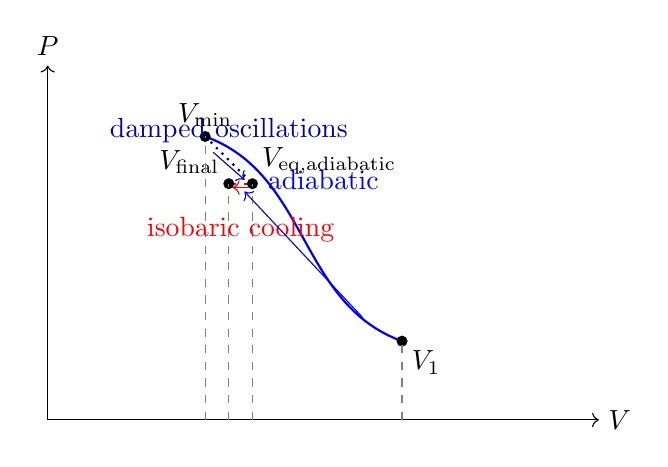
\begin{tikzpicture}[scale=1.0]

  % Axes
  \draw[->] (0,0) -- (7,0) node[right] {$V$};
  \draw[->] (0,0) -- (0,4.5) node[above] {$P$};

  % Adiabatic compression: V1 -> Vmin
  \draw[thick,blue]
    (4.5,1.0) to[out=160,in=-20] (2.0,3.6);

  % Relaxation (damped oscillations): Vmin -> V_eq
  \draw[thick,blue!70!black,dotted]
    (2.0,3.6) -- (2.6,3.0);

  % Isobaric cooling: V_eq -> V_final (horizontal line)
  \draw[thick,red,dashed]
    (2.6,3.0) -- (2.3,3.0);

  % Points
  \fill (4.5,1.0) circle (2pt) node[below right] {$V_1$};
  \fill (2.0,3.6) circle (2pt) node[above] {$V_{\min}$};
  \fill (2.6,3.0) circle (2pt) node[above right] {$V_{\text{eq,adiabatic}}$};
  \fill (2.3,3.0) circle (2pt) node[above left] {$V_{\text{final}}$};

  % Vertical guides
  \draw[gray,dashed] (4.5,0) -- (4.5,1.0);
  \draw[gray,dashed] (2.0,0) -- (2.0,3.6);
  \draw[gray,dashed] (2.6,0) -- (2.6,3.0);
  \draw[gray,dashed] (2.3,0) -- (2.3,3.0);

  % Labels
  \node[blue,above] at (3.5,2.8) {adiabatic};
  \node[blue!70!black,above] at (2.3,3.4) {damped oscillations};
  \node[red,below] at (2.45,2.7) {isobaric cooling};

  % Arrows (process directions)
  \draw[->,blue,thin] (4.0,1.3) -- (2.5,2.9);        % V1 -> Vmin
  \draw[->,blue!70!black,thin] (2.1,3.4) -- (2.5,3.05); % Vmin -> V_eq
  \draw[->,red,thin] (2.55,2.95) -- (2.35,2.95);     % V_eq -> V_final

\end{tikzpicture}
\end{center}

\begin{center}
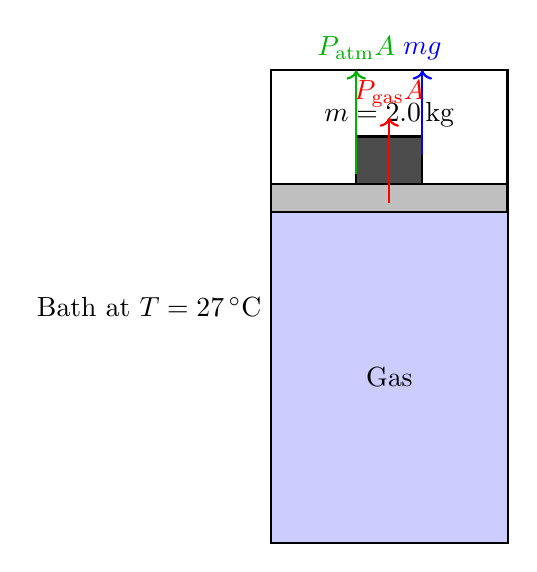
\begin{tikzpicture}[scale=1.2]
  % Cylinder walls
  \draw[thick] (0,0) rectangle (2.5,5);
  % Piston
  \draw[thick,fill=gray!50] (0,3.5) rectangle (2.5,3.8);
  % Mass on piston
  \draw[thick,fill=black!70] (0.9,3.8) rectangle (1.6,4.3);
  \node[above] at (1.25,4.3) {$m = \SI{2.0}{kg}$};

  % Gas below piston
  \draw[fill=blue!20] (0,0) rectangle (2.5,3.5);
  \node at (1.25,1.75) {Gas};

  % Forces - upward (gas pressure)
  \draw[->,red,thick] (1.25,3.6) -- (1.25,4.5) node[above] {$P_{\text{gas}}A$};

  % Forces - downward
  \draw[->,blue,thick] (1.6,4.1) -- (1.6,5.0) node[above] {$mg$};
  \draw[->,green!70!black,thick] (0.9,3.9) -- (0.9,5.0)
    node[above] {$P_{\text{atm}}A$};

  % Bath label
  \node[left] at (0,2.5) {Bath at $T = \SI{27}{\degreeCelsius}$};

\end{tikzpicture}
\end{center}

%%%%%%%%%%%%%%%%%%%%%%%%%%%%%%%%%%%%%%%%%%%%%%%%%%%%%%%%
\section*{Q9. A cycle with N\textsubscript{2} (3+3+2+3 pts)}

Given: \(n = 2\,\text{mol}\) N\textsubscript{2} (\(\gamma = 7/5\)),
\(T_A = \SI{300}{K}\),
\(V_A = \SI{0.0100}{m^3}\),
\(V_B = \SI{5}{L} = \SI{0.0050}{m^3}\),
\(T_C = \SI{300}{K}\).

\subsection*{(a) Net work}
\textbf{Process A→B (adiabatic compression):}
\[
T_B = T_A \left(\frac{V_A}{V_B}\right)^{\gamma-1}
= 300 \times \left(\frac{0.0100}{0.0050}\right)^{0.4}
= 300 \times 2^{0.4} = \SI{396}{K}.
\]

\[
W_{AB} = \frac{nR}{\gamma-1}(T_A - T_B)
= \frac{2 \times 8.314}{0.4}(300 - 396)
= \ans{\SI{-3.98e3}{J}}.
\]

\textbf{Process B→C (isochoric):} \(W_{BC} = 0\).

\textbf{Process C→A (isothermal expansion):}
\[
W_{CA} = nRT_C \ln\frac{V_A}{V_C}
= 2 \times 8.314 \times 300 \times \ln\frac{0.0100}{0.0050}
= \ans{\SI{3.46e3}{J}}.
\]

Net work: \(W_{\text{net}} = W_{AB} + W_{BC} + W_{CA} = -3985 + 0 + 3458 = \ans{\SI{-527}{J}}\).

\subsection*{(b) Net heat}
From first law: \(Q_{\text{net}} = W_{\text{net}} = \ans{\SI{-527}{J}}\) (since \(\Delta U_{\text{cycle}} = 0\)).

\subsection*{(c) Change in internal energy}
\[
\Delta U_{\text{cycle}} = \ans{0}.
\]

\subsection*{(d) Entropy change}
For a complete cycle: \(\Delta S_{\text{cycle}} = \ans{0}\) (entropy is a state function).

\noindent\textbf{Required drawing:}
\begin{center}
  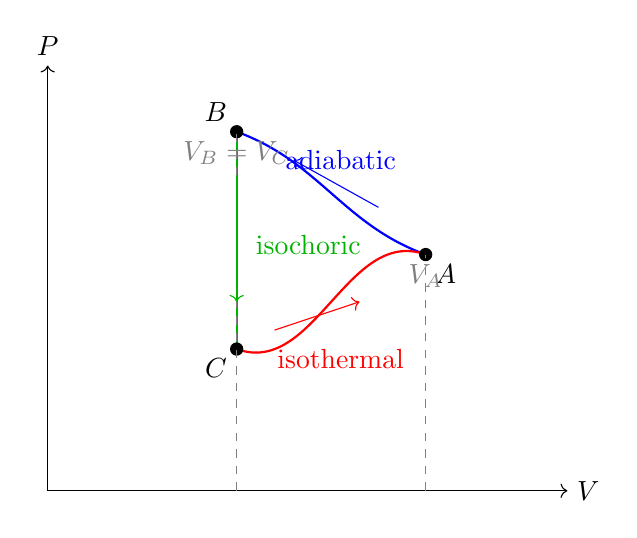
\begin{tikzpicture}[scale=1.2]
    % Axes
    \draw[->] (0,0) -- (5.5,0) node[right] {$V$};
    \draw[->] (0,0) -- (0,4.5) node[above] {$P$};
  
    % Adiabatic A->B (compression)
    \draw[thick,blue]
      (4.0,2.5) to[out=160,in=-20] (2.0,3.8);
  
    % Isochoric B->C (vertical down)
    \draw[thick,green!70!black]
      (2.0,3.8) -- (2.0,1.5);
  
    % Isothermal C->A (gentle curve back)
    \draw[thick,red]
      (2.0,1.5) to[out=-20,in=160] (4.0,2.5);
  
    % Points A, B, C
    \fill (4.0,2.5) circle (2pt) node[below right] {$A$};
    \fill (2.0,3.8) circle (2pt) node[above left] {$B$};
    \fill (2.0,1.5) circle (2pt) node[below left] {$C$};
  
    % Rough volume labels
    \draw[gray,dashed] (4.0,0) -- (4.0,2.5) node[below] {$V_A$};
    \draw[gray,dashed] (2.0,0) -- (2.0,3.8) node[below] {$V_B=V_C$};
  
    % Process labels
    \node[blue,above] at (3.1,3.3) {adiabatic};
    \node[green!70!black,right] at (2.1,2.6) {isochoric};
    \node[red,below] at (3.1,1.6) {isothermal};
  
    % Direction arrows (A -> B -> C -> A)
    \draw[->,blue,thin] (3.5,3.0) -- (2.6,3.5);
    \draw[->,green!70!black,thin] (2.0,3.3) -- (2.0,2.0);
    \draw[->,red,thin] (2.4,1.7) -- (3.3,2.0);
  \end{tikzpicture}
  \end{center}

%%%%%%%%%%%%%%%%%%%%%%%%%%%%%%%%%%%%%%%%%%%%%%%%%%%%%%%%
\section*{Q10. Carnot engine with N\textsubscript{2} (4+4+3+3+1+3 pts)}

Given: \(n = 1\,\text{mol}\) N\textsubscript{2},
\(T_h = \SI{400}{K}\),
\(T_c = \SI{300}{K}\),
\(V_a = \SI{6.0}{L} = \SI{0.0060}{m^3}\),
\(V_c = \SI{18.0}{L} = \SI{0.0180}{m^3}\),
\(\gamma = 7/5\).

\subsection*{(a) Volume \(V_b\)}
At state \(b\), isothermal expansion ends. For adiabatic process b→c:
\[
T_h V_b^{\gamma-1} = T_c V_c^{\gamma-1}
\quad\Rightarrow\quad
V_b = V_c \left(\frac{T_c}{T_h}\right)^{1/(\gamma-1)}.
\]
\[
V_b = 0.0180 \times \left(\frac{300}{400}\right)^{5/2}
= 0.0180 \times 0.75^{2.5}
= 0.0180 \times 0.4867
= \ans{\SI{0.00877}{m^3} = \SI{8.77}{L}}.
\]

\subsection*{(b) Volume \(V_d\)}
At state \(d\), adiabatic compression ends. For adiabatic process d→a:
\[
T_c V_d^{\gamma-1} = T_h V_a^{\gamma-1}
\quad\Rightarrow\quad
V_d = V_a \left(\frac{T_h}{T_c}\right)^{1/(\gamma-1)}.
\]
\[
V_d = 0.0060 \times \left(\frac{400}{300}\right)^{5/2}
= 0.0060 \times 1.333^{2.5}
= \ans{\SI{0.0123}{m^3} = \SI{12.3}{L}}.
\]

\subsection*{(c) Heat input \(Q_{\text{in}}\)}
For isothermal expansion a→b:
\[
Q_{\text{in}} = nRT_h \ln\frac{V_b}{V_a}
= 1 \times 8.314 \times 400 \times \ln\frac{0.00877}{0.0060}
= \ans{\SI{1.26e3}{J}}.
\]

\subsection*{(d) Heat out \(Q_{\text{out}}\)}
For isothermal compression c→d:
\[
Q_{\text{out}} = -nRT_c \ln\frac{V_d}{V_c}
= -1 \times 8.314 \times 300 \times \ln\frac{0.0123}{0.0180}
= \ans{\SI{950}{J}}.
\]

\subsection*{(e) Efficiency}
\[
\eta = 1 - \frac{T_c}{T_h} = 1 - \frac{300}{400} = \ans{0.25 = 25\%}.
\]

\subsection*{(f) Entropy change per gram}
Molar mass of N\textsubscript{2}: \(M = \SI{28}{g/mol}\).

\textbf{Process a→b (isothermal):}
Using \(V_b = \SI{0.008769}{m^3}\) (from part (a)):
\[
\Delta S_{ab} = nR \ln\frac{V_b}{V_a} = 1 \times 8.314 \times \ln\frac{0.008769}{0.0060} = \SI{3.154}{J/K}.
\]

Per gram: \(\frac{\Delta S_{ab}}{M} = \frac{3.154}{28} = \ans{\SI{0.113}{J/(K\cdot g)}}\).

\textbf{Process b→c (adiabatic):} \(\Delta S_{bc} = 0\), so per gram: \ans{0}.

\noindent\textbf{Required drawing:}
\begin{center}
  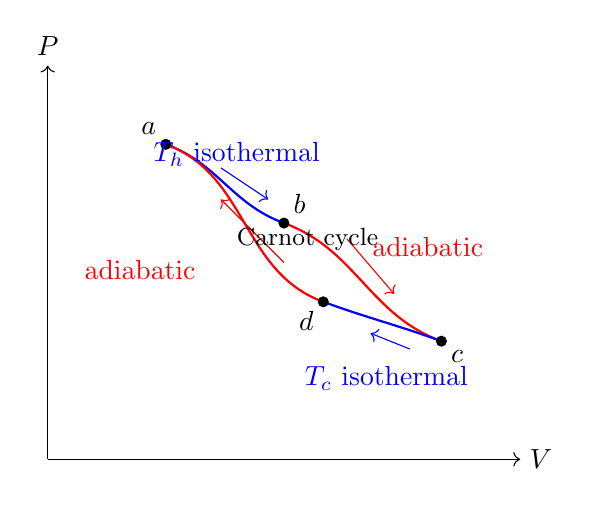
\begin{tikzpicture}[scale=1.0]
    % Axes
    \draw[->] (0,0) -- (6,0) node[right] {$V$};
    \draw[->] (0,0) -- (0,5) node[above] {$P$};
  
    % Isothermal expansion a->b at Th
    \draw[thick,blue]
      (1.5,4.0) to[out=-20,in=160] (3.0,3.0);
  
    % Adiabatic expansion b->c
    \draw[thick,red]
      (3.0,3.0) to[out=-20,in=160] (5.0,1.5);
  
    % Isothermal compression c->d at Tc
    \draw[thick,blue]
      (5.0,1.5) to[out=160,in=-20] (3.5,2.0);
  
    % Adiabatic compression d->a
    \draw[thick,red]
      (3.5,2.0) to[out=160,in=-20] (1.5,4.0);
  
    % Points a, b, c, d
    \fill (1.5,4.0) circle (2pt) node[above left] {$a$};
    \fill (3.0,3.0) circle (2pt) node[above right] {$b$};
    \fill (5.0,1.5) circle (2pt) node[below right] {$c$};
    \fill (3.5,2.0) circle (2pt) node[below left] {$d$};
  
    % Process labels
    \node[blue,above] at (2.4,3.6) {$T_h$ isothermal};
    \node[red,right] at (4.0,2.7) {adiabatic};
    \node[blue,below] at (4.3,1.3) {$T_c$ isothermal};
    \node[red,left] at (2.0,2.4) {adiabatic};
  
    % Direction arrows (Carnot direction a -> b -> c -> d -> a)
    \draw[->,blue,thin] (2.2,3.7) -- (2.8,3.3);
    \draw[->,red,thin]  (3.8,2.8) -- (4.4,2.1);
    \draw[->,blue,thin] (4.6,1.4) -- (4.1,1.6);
    \draw[->,red,thin]  (3.0,2.5) -- (2.2,3.3);
  
    \node at (3.3,2.8) {\small Carnot cycle};
  \end{tikzpicture}
  \end{center}

%%%%%%%%%%%%%%%%%%%%%%%%%%%%%%%%%%%%%%%%%%%%%%%%%%%%%%%%
\section*{Bonus. Greenhouse effect (0--2 pts)}

The greenhouse effect occurs when certain atmospheric gases (e.g., CO\textsubscript{2}, water vapor, methane) absorb and re-emit infrared radiation emitted by Earth's surface, trapping heat and warming the planet. Without this effect, Earth's average temperature would be about \SI{255}{K}, but the actual mean surface temperature is \SI{288}{K}, demonstrating its importance.

To make Earth a better place to live:
\begin{enumerate}
\item Reduce greenhouse gas emissions by transitioning to renewable energy sources and improving energy efficiency.
\item Protect and restore natural carbon sinks like forests and oceans that absorb CO\textsubscript{2}.
\item Develop and deploy carbon capture technologies to remove excess CO\textsubscript{2} from the atmosphere.
\end{enumerate}

\section*{Assistance notes:} LLMs were used as translators and concept explainers. No direct solutions were provided.

\end{document}


